% 中山大学科技类及IT类实验报告文档类(LaTeX模板)
\documentclass{sysucseexp}
\usepackage{fontspec,inconsolata,url}
\setmainfont{Times New Roman}
\setmonofont{Consolas}

% 载入需要的宏包
\input{settings/packages.tex}
% 进行必要的设置
\input{settings/format.tex}
% 专用术语宏命令进行必要的设置
\input{settings/terms.tex}

% 设置封面基本信息
\sysucseset{
  college = {计算机学院},
  projname = {计算复杂性理论实验},
  title = {第一次编程作业},
  stunoleader = {23336150},
  authorleader = {刘昊},
  stunoone = {23336203},
  authorone = {任意嵘},
  stunotwo = {23336193},
  authortwo = {彭怡萱},
  major = {计算机科学与技术},
  adviser = {冯剑琳},
  startdate = {2026年3月23日},
  enddate = {4月3日}
}

\begin{document}

% 封面及目录
\makecover
\tableofcontents
\cleardoublepage
\pagestyle{main}

%%%%%%%%%%%%%%%%%%%%%%%%%%%%%%%%%%%%%%%%

\section{实验目的与要求}

本次编程作业要求以小组为单位，编写 Python 程序实现图灵机编码、多带图灵机以及通用图灵机，并以两数加法图灵机 ADD 为测试用例进行测试。

\textbf{项目已完成所有模块的实现}，具体要求如下：

\begin{enumerate}
    \item \textbf{图灵机编码模块}：读取 JSON 文件并转换为二进制编码，将状态、符号、方向映射为正整数后用一进制表示。

    \item \textbf{多带图灵机模块}：实现多带图灵机模拟器，支持交互式和自动两种展示模式，实时打印磁带状态和磁头位置。

    \item \textbf{通用图灵机模块}：基于多带图灵机实现 UTM，使用三条磁带模拟任意单带图灵机，打印运行阶段说明。

    \item \textbf{用例测试}：构造 ADD 图灵机的 JSON 定义文件，执行 UTM 运转测试。
\end{enumerate}

\section{模块设计思路}

\subsection{图灵机编码模块}

编码模块将图灵机的 JSON 定义转换为二进制字符串。设计过程分为以下步骤：

\textbf{步骤1：JSON 解析与归一化}

读取 JSON 后遍历每个状态及其转移条件，校验核心字段是否存在。同时对符号和方向进行归一化处理，例如将空白符的多种写法统一为单空格，将方向统一为 \texttt{left}、\texttt{right}、\texttt{stay}。

\textbf{步骤2：状态 ID 映射}

采用两阶段映射策略避免 ID 冲突：首先用正则表达式提取符合 \texttt{qN} 格式的状态编号；然后对非标准状态按字典序分配剩余的最小正整数。

\textbf{步骤3：符号与方向 ID 分配}

按照规范固定分配：\texttt{0}$\rightarrow$1，\texttt{1}$\rightarrow$2，空格$\rightarrow$3，其余符号从4开始递增。方向映射为：\texttt{left}$\rightarrow$1，\texttt{right}$\rightarrow$2，\texttt{stay}$\rightarrow$3。

\textbf{步骤4：转移排序与编码}

为保证编码确定性，对转移规则按五维键值排序后，将每个转移编码为一进制串，转移内部用 \texttt{1} 分隔，转移之间用 \texttt{11} 连接。

% 图片位置：图灵机编码流程图
% \begin{figure}[H]
%     \centering
%     % \includegraphics[width=0.8\textwidth]{figs/编码流程图.png}
%     \fbox{\parbox{0.8\textwidth}{\centering\vspace{2cm}【图片占位：图灵机编码流程图】\vspace{2cm}}}
%     \caption{图灵机编码模块工作流程}
%     \label{fig:encoding_flow}
% \end{figure}

\subsection{多带图灵机模块}

多带图灵机模块实现了一个通用的模拟器，设计过程如下：

\textbf{步骤1：磁带模型设计}

每条磁带用字符列表表示，支持双向无限延伸。磁头位置用整数索引标记，读写操作自动处理边界扩展。

\textbf{步骤2：转移规则定义}

转移规则基于当前状态和所有磁带的读取符号，确定写入符号、移动方向和下一状态。使用元组作为字典键实现高效查找。

\textbf{步骤3：执行流程实现}

每步执行时：读取所有磁头符号 $\rightarrow$ 查找匹配转移 $\rightarrow$ 执行写入和移动 $\rightarrow$ 更新状态。支持交互式（等待用户输入）和自动模式（固定时间间隔）。

% 图片位置：多带图灵机结构示意图
% \begin{figure}[H]
%     \centering
%     % \includegraphics[width=0.9\textwidth]{figs/多带图灵机结构.png}
%     \fbox{\parbox{0.9\textwidth}{\centering\vspace{2cm}【图片占位：多带图灵机结构示意图】\vspace{2cm}}}
%     \caption{多带图灵机的磁带与磁头结构}
%     \label{fig:multitape_structure}
% \end{figure}

\subsection{通用图灵机模块}

UTM 模块基于多带图灵机实现，按照 \texttt{tm2.ppt} 的定义设计：

\textbf{步骤1：三带架构设计}

\begin{itemize}
    \item \textbf{Tape 1}：存储被模拟图灵机的编码 $M$ 和输入 $w$，格式为 $M111w$
    \item \textbf{Tape 2}：模拟被模拟图灵机的磁带，符号用一进制编码表示
    \item \textbf{Tape 3}：存储被模拟图灵机的当前状态（状态ID的一进制）
\end{itemize}

\textbf{步骤2：编码解析}

从 Tape 1 解析转移规则：用 \texttt{11} 分隔各转移，用 \texttt{1} 分隔转移内部各部分，读取连续 \texttt{0} 的数量得到数值。

\textbf{步骤3：执行阶段实现}

按照标准步骤执行：Step 2 分析符号表示长度 $\rightarrow$ Step 3 初始化磁带 $\rightarrow$ 主循环查找并执行转移 $\rightarrow$ 判断接受或拒绝。

% 图片位置：UTM三带架构图
% \begin{figure}[H]
%     \centering
%     % \includegraphics[width=0.9\textwidth]{figs/UTM三带架构.png}
%     \fbox{\parbox{0.9\textwidth}{\centering\vspace{2cm}【图片占位：UTM三带架构示意图】\vspace{2cm}}}
%     \caption{通用图灵机的三带架构}
%     \label{fig:utm_architecture}
% \end{figure}

\section{关键代码展示}

\subsection{图灵机编码模块}

\subsubsection{转移规则排序}

为保证编码结果的确定性，对转移规则按五维键值进行排序：

\begin{lstlisting}[language=Python]
ordered_transitions = sorted(
    transitions,
    key=lambda transition: (
        state_ids[transition.current_state],
        symbol_ids[transition.read_symbol],
        state_ids[transition.next_state],
        symbol_ids[transition.write_symbol],
        DIRECTION_IDS[transition.move],
    ),
)
\end{lstlisting}

排序后，无论 JSON 中状态的书写顺序如何，同一图灵机始终产生相同的编码字符串。

\subsubsection{状态 ID 映射}

采用两阶段策略避免 ID 冲突：

\begin{lstlisting}[language=Python]
def build_state_ids(transitions):
    # 阶段1：提取 qN 格式的状态编号
    for state_name in sorted(state_names):
        match = STATE_NAME_PATTERN.fullmatch(state_name)
        if match:
            state_ids[state_name] = int(match.group(1))
    
    # 阶段2：为非标准状态分配剩余ID
    for state_name in sorted(state_names):
        if state_name not in state_ids:
            state_ids[state_name] = next_available
            next_available += 1
\end{lstlisting}

\subsubsection{一进制编码}

将转移规则转换为一进制字符串：

\begin{lstlisting}[language=Python]
def encode_transition(transition, state_ids, symbol_ids):
    parts = [
        unary_encode(state_ids[transition.current_state]),
        unary_encode(symbol_ids[transition.read_symbol]),
        unary_encode(state_ids[transition.next_state]),
        unary_encode(symbol_ids[transition.write_symbol]),
        unary_encode(DIRECTION_IDS[transition.move]),
    ]
    return "1".join(parts)  # 转移内部用1分隔
\end{lstlisting}

最终将所有转移用 \texttt{11} 连接：\texttt{"11".join(encodings)}。

\subsection{多带图灵机模块}

\subsubsection{磁带类实现}

磁带类封装了读写和移动操作：

\begin{lstlisting}[language=Python]
class Tape:
    def __init__(self):
        self.content = [" "]  # 初始为空符号
        self.head_position = 0
    
    def read(self) -> str:
        return self.content[self.head_position]
    
    def write(self, symbol: str):
        self.content[self.head_position] = symbol
    
    def move(self, direction: str):
        if direction == "left":
            self.head_position -= 1
        elif direction == "right":
            self.head_position += 1
\end{lstlisting}

磁带自动处理边界扩展，支持无限延伸。

\subsubsection{单步执行}

核心的 \texttt{step()} 方法实现单步转移：

\begin{lstlisting}[language=Python]
def step(self) -> bool:
    if self.halted:
        return False
    
    # 读取所有磁带的当前符号
    current_symbols = tuple(tape.read() for tape in self.tapes)
    key = (self.current_state, current_symbols)
    
    # 查找匹配的转移规则
    if key not in self.transitions:
        self.halted = True
        return False
    
    # 执行转移
    transition = self.transitions[key]
    for i, tape in enumerate(self.tapes):
        tape.write(transition.write_symbols[i])
        tape.move(transition.moves[i])
    
    self.current_state = transition.next_state
    return True
\end{lstlisting}

\subsection{通用图灵机模块}

\subsubsection{磁带初始化}

UTM 初始化时设置三条磁带的内容：

\begin{lstlisting}[language=Python]
def initialize_tapes(self):
    # Tape1: M111w
    tape1_content = self.machine_encoding + "111" + self.input_string
    self.tapes[0].content = list(tape1_content)
    
    # Tape2: 输入w的符号编码
    tape2_content = self._encode_input_for_tape2(self.input_string)
    self.tapes[1].content = list(tape2_content)
    
    # Tape3: 起始状态编码
    start_encoding = self._unary_encode(self.simulated_state_id)
    self.tapes[2].content = list(start_encoding)
\end{lstlisting}

\subsubsection{转移解析}

从编码字符串解析转移规则：

\begin{lstlisting}[language=Python]
def _parse_transitions(self, encoding: str):
    transitions = []
    for part in encoding.split("11"):  # 转移间用11分隔
        components = part.split("1")    # 转移内部用1分隔
        if len(components) == 5:
            transition = UTMTransition(
                current_state_id=len(components[0]),  # 0的数量
                read_symbol_id=len(components[1]),
                next_state_id=len(components[2]),
                write_symbol_id=len(components[3]),
                move_id=len(components[4])
            )
            transitions.append(transition)
    return transitions
\end{lstlisting}

\subsubsection{主循环执行}

UTM 的主循环实现：

\begin{lstlisting}[language=Python]
def step(self) -> bool:
    if self.state.halted:
        return False
    
    # 解码当前符号
    current_symbol_id = self._decode_symbol_from_tape2()
    
    # 搜索匹配转移
    self.state.stage = "search_move"
    transition = self._find_matching_transition(
        self.simulated_state_id, current_symbol_id)
    
    if transition is None:
        self.state.stage = "no_match"
        self.state.halted = True
        return False
    
    # 执行转移
    self.state.stage = "execute_move"
    self._execute_transition(transition)
    
    return True
\end{lstlisting}

\section{运行结果展示}

\subsection{图灵机编码模块测试}

运行程序选择编码功能，对 ADD 图灵机进行编码：

\begin{lstlisting}[language=bash]
$ python main.py encode --sample add_tm.json --details
\end{lstlisting}

编码结果输出状态映射、符号映射和转移规则列表：

% 图片位置：编码结果截图
\begin{figure}[H]
    \centering
    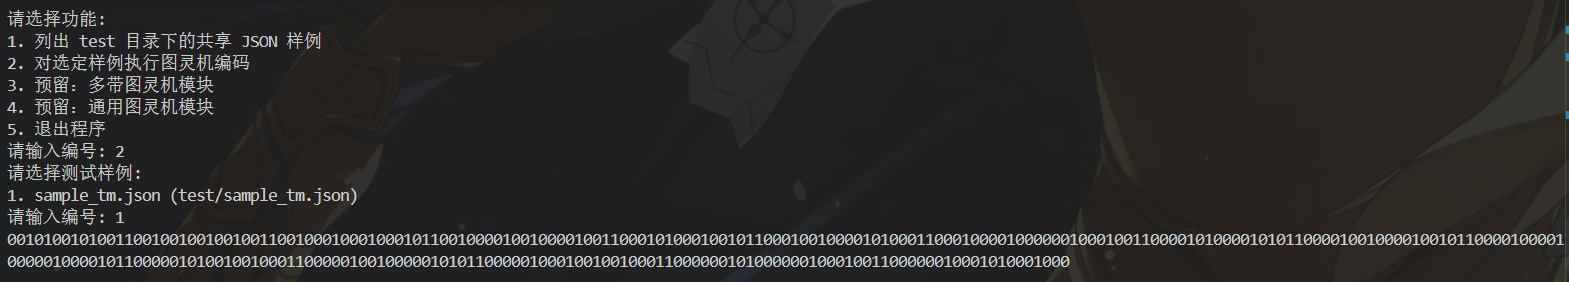
\includegraphics[width=0.9\textwidth]{figs/图灵机编码结果演示.png}
    \caption{ADD图灵机编码结果}
    \label{fig:encode_result}
\end{figure}

编码成功生成 21 个转移规则，状态映射为 q1$\rightarrow$1, q2$\rightarrow$2, ..., halt$\rightarrow$8，符号映射为 0$\rightarrow$1, 1$\rightarrow$2, 空格$\rightarrow$3。

\subsection{多带图灵机模块测试}

使用两带图灵机示例进行测试：

\begin{lstlisting}[language=bash]
$ python main.py multitape --mode auto --interval 0.1
\end{lstlisting}

运行过程展示每步的状态变化：

\begin{lstlisting}[language=bash]
============================================================
多带图灵机模拟器
============================================================
初始状态
当前状态：q1    步数：0
Tape 1:      *0101
Tape 2:      *

第 1 步
当前状态：q1    步数：1
Tape 1:      0*101
Tape 2:      *

...

第 7 步
当前状态：halt    步数：7
Tape 1:      0*110
Tape 2:      *

结果：接受 (ACCEPTED)
总步数：7
============================================================
\end{lstlisting}

% 图片位置：多带图灵机运行截图
\begin{figure}[H]
    \centering
    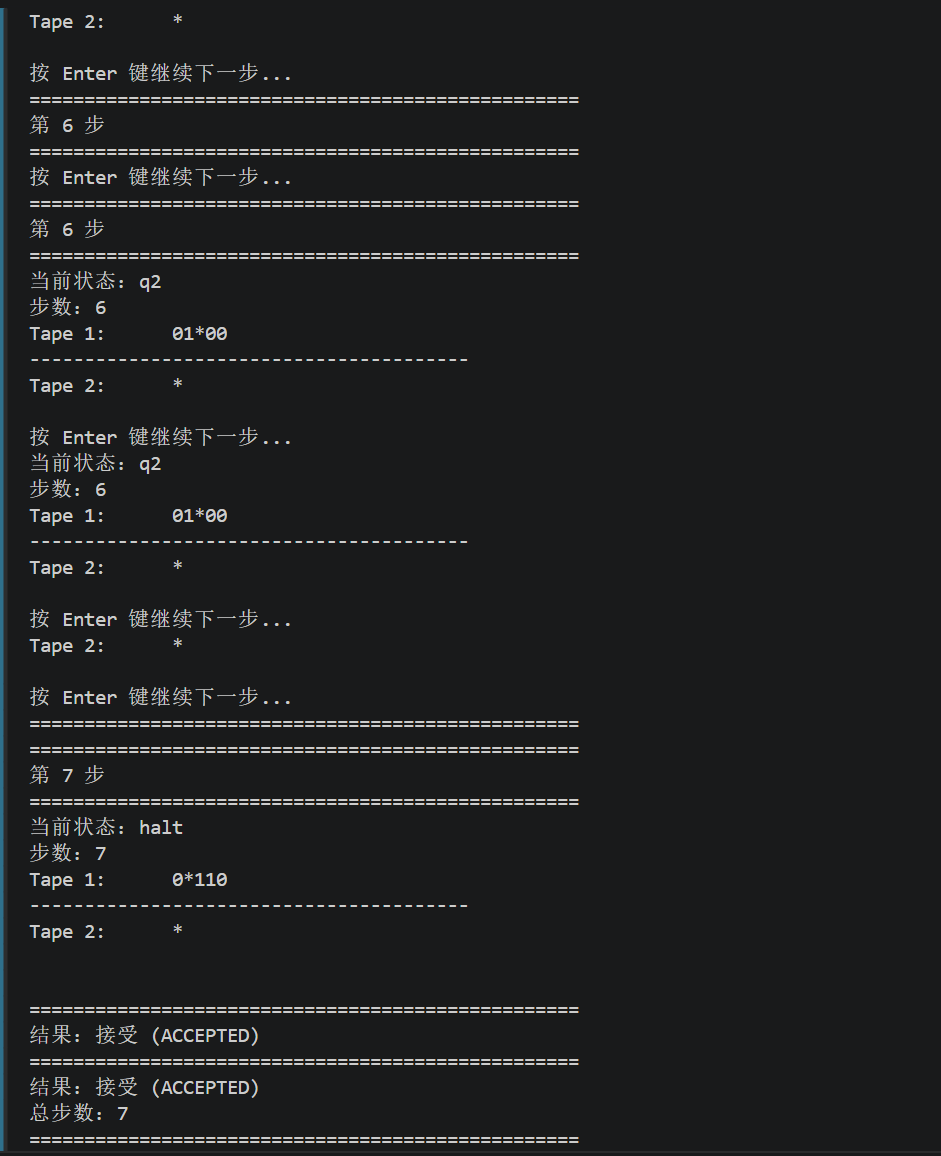
\includegraphics[width=0.9\textwidth]{figs/多带图灵机运行.png}
    % \fbox{\parbox{0.9\textwidth}{\centering\vspace{2cm}【图片占位：多带图灵机完整运行截图】\vspace{2cm}}}
    \caption{多带图灵机运行过程（部分截图）}
    \label{fig:multitape_run}
\end{figure}

\subsection{通用图灵机模块测试}

使用 ADD 图灵机测试 UTM：

\begin{lstlisting}[language=bash]
$ python main.py utm --sample add_tm.json --mode auto
\end{lstlisting}

UTM 初始化阶段输出：

\begin{lstlisting}[language=bash]
============================================================
UTM 初始化
============================================================
当前阶段说明：Step 2: The UTM examines M to see how many 
of its own tape squares it needs to represent one symbol of M.
符号表示长度：8 个UTM符号

当前阶段说明：Step 3: Initialize Tape 2 to represent the 
tape of M with input w, and initialize Tape 3 to hold the 
start state.
\end{lstlisting}

% 图片位置：UTM初始化截图
\begin{figure}[H]
    \centering
    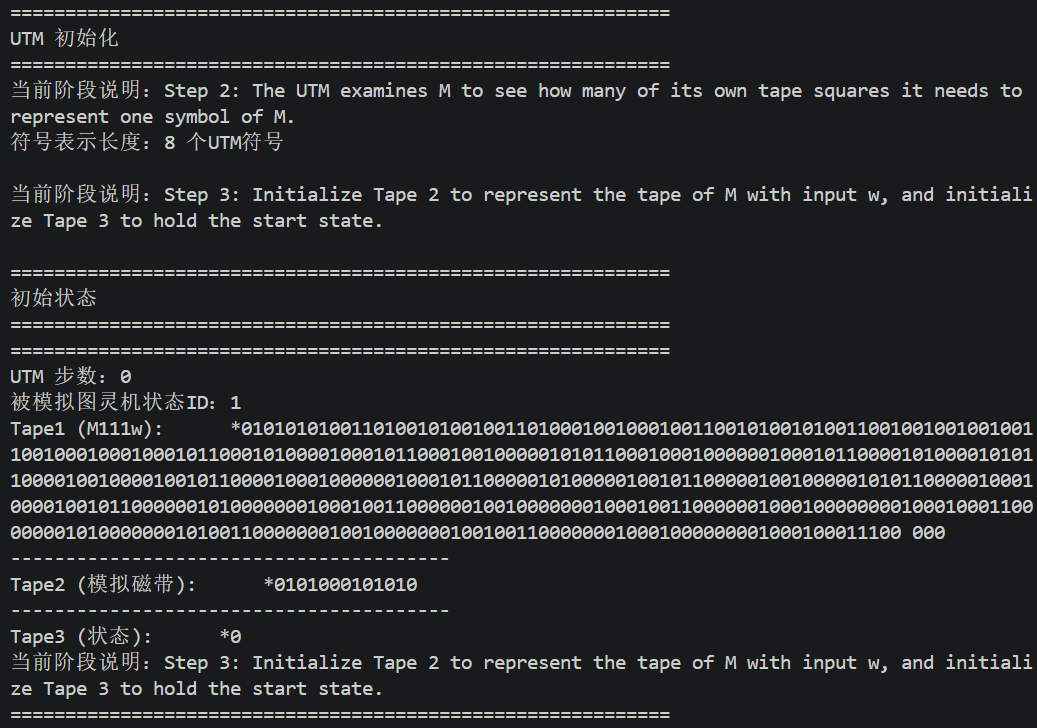
\includegraphics[width=0.9\textwidth]{figs/UTM初始化.png}
    % \fbox{\parbox{0.9\textwidth}{\centering\vspace{2cm}【图片占位：UTM初始化状态截图】\vspace{2cm}}}
    \caption{UTM初始化阶段}
    \label{fig:utm_init}
\end{figure}

运行过程展示三条磁带的状态变化：

\begin{lstlisting}[language=bash]
UTM 步数：0
被模拟图灵机状态ID：1
Tape1 (M111w):      *01010101...11100 000
Tape2 (模拟磁带):      *0101000101010
Tape3 (状态):      *0

UTM 步数：6
被模拟图灵机状态ID：8
Tape1 (M111w):      *01010101...11100 000
Tape2 (模拟磁带):      000*1   101010
Tape3 (状态):      *00000000
当前阶段说明：M accepts, the UTM also accepts.

结果：接受 (ACCEPTED)
总步数：6
\end{lstlisting}

% 图片位置：UTM运行截图
\begin{figure}[H]
    \centering
    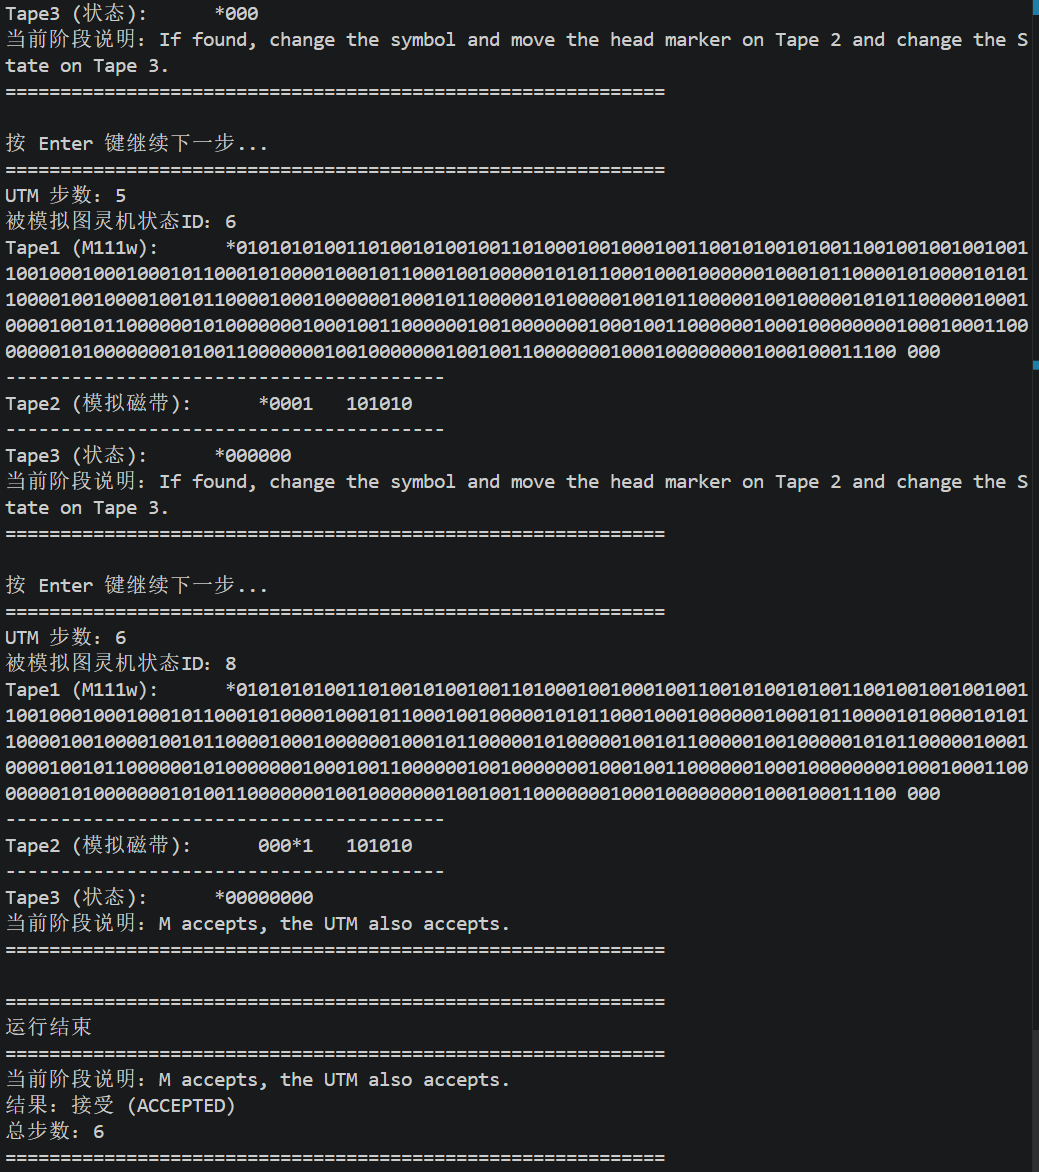
\includegraphics[width=0.9\textwidth]{figs/UTM运行.png}
    % \fbox{\parbox{0.9\textwidth}{\centering\vspace{2cm}【图片占位：UTM完整运行截图】\vspace{2cm}}}
    \caption{UTM运行过程（部分截图）}
    \label{fig:utm_run}
\end{figure}

UTM 成功在 6 步后接受，验证了 ADD 图灵机对输入 2+3 的正确计算。

\section{总结}

本项目成功实现了图灵机编码、多带图灵机和通用图灵机三个模块。编码模块采用确定性排序保证编码唯一性；多带图灵机模块支持任意数量磁带和两种运行模式；UTM 模块按照标准定义实现三带架构，能够模拟任意单带图灵机。所有模块通过 ADD 图灵机测试验证了正确性。

\end{document}
